\subsection{Charge-Pump Branch and DC Link}
\label{sec:hw-pump}

The charge-pump branch connects the rectified line to VSW and the high-voltage DC link. In the V2 drawing, C24 is the \SI{2}{\nano\farad} pump capacitor, L3 is the pump-path inductance, and D6--D8 steer charge into the link. The isolated resonant path also starts at VSW, so the same half bridge drives input-current shaping and power transfer.

A KEMET C1206X202FBGACTU pump capacitor was used, rated \SI{2000}{\pico\farad}, \SI{630}{\volt}, \(\pm1\%\), C0G/NP0 \cite{kemetC1206X202FBGACTU}. Its capacitance sets the charge moved in each cycle. The component list specifies PU1JLWH \SI{600}{\volt}, \SI{1}{\ampere} ultrafast pump rectifiers \cite{taiwansemiPU1JLWH} and a Wurth Elektronik 860241478004 \SI{22}{\micro\farad}, \SI{450}{\volt} DC-link capacitor \cite{wurth860241478004}. C25 is specified as \SI{22}{\micro\farad} in V1.0 and \SI{10}{\micro\farad} in V1.1. The component list and V1.0 board value describe the tested link.

The branch carries pulsed current as the line voltage changes. The operating margin still needs to be checked by measuring peak and RMS diode current, capacitor current, DC-link ripple and peak voltage, and loop overshoot. The results can then be compared with the part ratings.

\begin{landscape}
\begin{figure}[htbp]
\centering
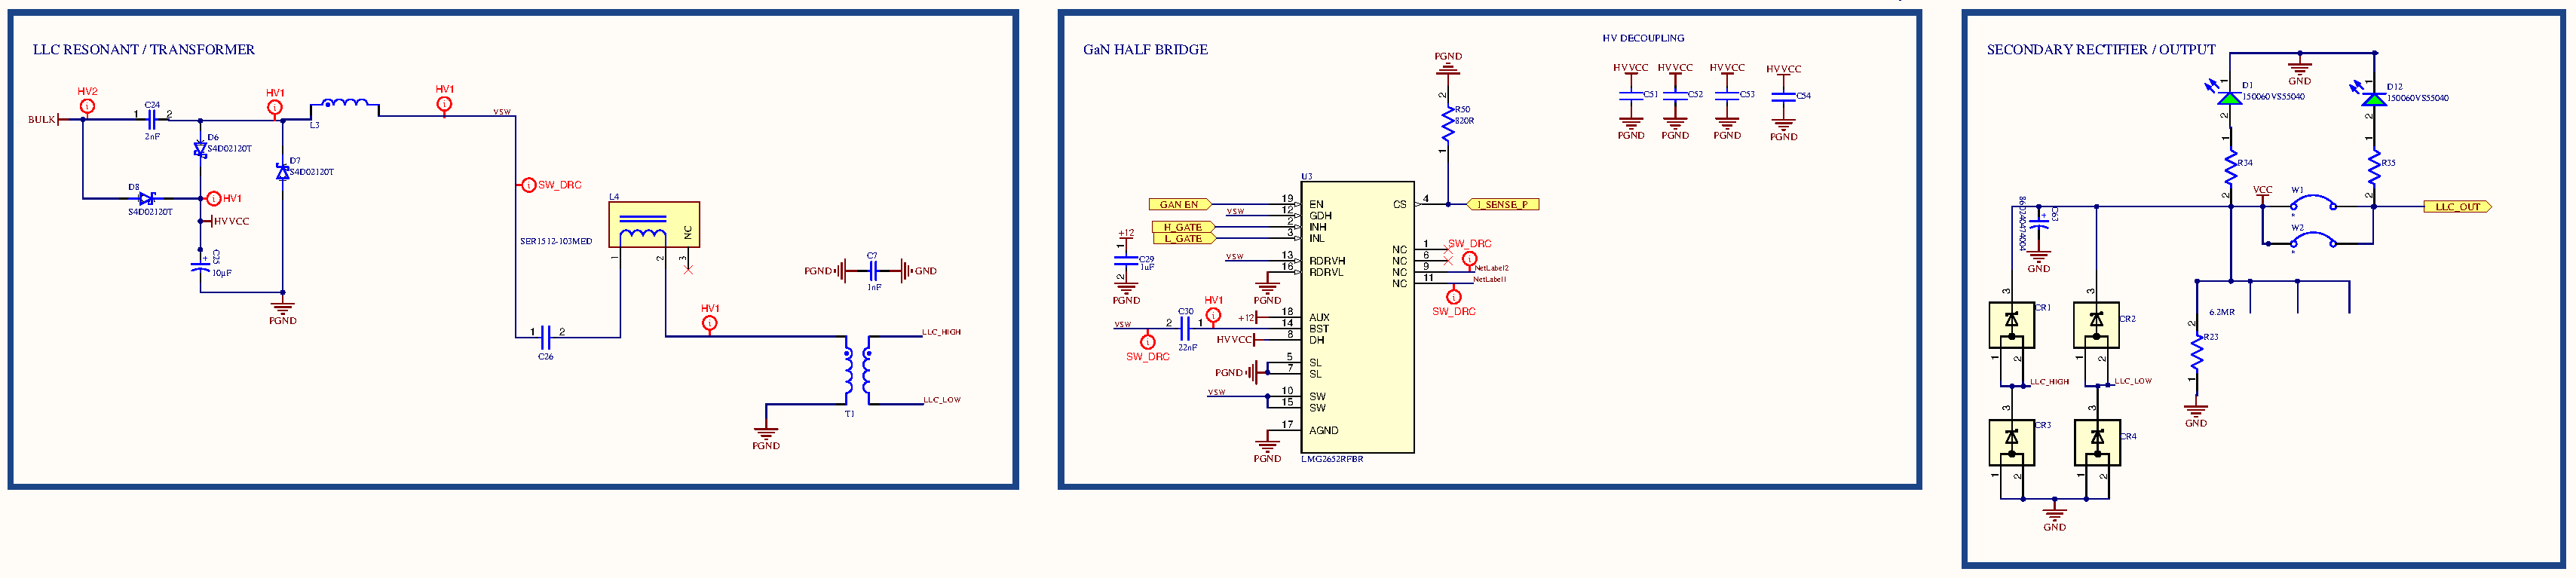
\includegraphics[width=0.98\linewidth,height=0.77\textheight,keepaspectratio]{Pictures/Thesis/07_Hardware/Rebuilt/schematic_v2_power_stage_excerpt.pdf}
\caption{V2 sheet 3 charge-pump and resonant power circuit. C24 and D6--D8 form the pump branch, the GaN half bridge drives the tank and transformer, and the secondary bridge supplies the isolated bulk output.}
\label{fig:schematic-power-stage}
\end{figure}
\end{landscape}
